\documentclass[a4paper 12pt]{article}

\usepackage[utf8]{inputenc}
\usepackage[T1]{fontenc}
\usepackage{mathptmx}
\usepackage{textcomp}
\usepackage[UKenglish]{babel}
\usepackage{amsmath, amssymb}
\usepackage{float}
\usepackage{xcolor}
\definecolor{codegreen}{rgb}{0,0.6,0}
\definecolor{codepurple}{rgb}{0.58,0,0.82}
\usepackage{listings}
\lstdefinestyle{code}{
	commentstyle=\color{codegreen},
	keywordstyle=\color{magenta},
	stringstyle=\color{codepurple},
	showspaces=false,
	showstringspaces=false,
	breaklines=true
}
\lstset{style=code}
\usepackage[hidelinks]{hyperref}
\hypersetup{
	colorlinks=false
}
\usepackage[style=ieee]{biblatex}
\bibliography{sources/biblio}
\renewcommand{\baselinestretch}{1.5}

\setlength{\parindent}{0pt}
\setlength{\parskip}{1em}

% figure support
\usepackage{import}
\usepackage{xifthen}
\pdfminorversion=7
\usepackage{pdfpages}
\usepackage{transparent}
\newcommand{\incfig}[1]{%
	\def\svgwidth{\columnwidth}
	\import{./figures/}{#1.pdf_tex}
}

\pdfsuppresswarningpagegroup=1

\begin{document}
\hypersetup{pageanchor=false}
\begin{titlepage}
  \begin{center}

    \textsc{\LARGE Dublin City University}\\[1cm]
    \textsc{\Large Electronic and Computer Engineering}\\[0.5cm]

    {\LARGE \bfseries EE515 Real-Time DSP: Assignment 1\\[0.4cm]}
    {\Large \bfseries The role of Digital Signal Processing in Optical
    Communications Systems\\[0.4cm]}

    \begin{figure}[H]
	
\includegraphics{images/Dcu-logo.png}
	\centering
    \end{figure}

    \vskip 2cm
    \emph{Author}\\[0.1cm]
    \noindent\makebox[\textwidth]{%
      \begin{tabular}{ll}%
        Michael Lenehan & michael.lenehan4@mail.dcu.ie \\
	Student Number: & 15410402 \\
    \end{tabular}}\\[0.1cm]

    \vfill

    % Bottom of the page
    % Probably replaced with date of deadline
    {\large{26/11/2019}}

  \end{center}
\end{titlepage}

\hypersetup{pageanchor=true}
\pagenumbering{alph}
\thispagestyle{plain}
\begingroup
\renewcommand{\cleardoublepage}{}
\renewcommand{\clearpage}{}

\LARGE{Declaration}

\endgroup

\vskip 1cm

I declare that this material, which I now submit for assessment, is entirely my
own work and has not been taken from the work of others, save and to the extent
that such work has been cited and acknowledged within the text of my work. I
understand that plagiarism, collusion, and copying are grave and serious
offences in the university and accept the penalties that would be imposed should
I engage in plagiarism, collusion or copying. I have read and understood the
Assignment Regulations set out in the module documentation. I have identified
and included the source of all facts, ideas, opinions, and viewpoints of others
in the assignment references. Direct quotations from books, journal articles,
internet sources, module text, or any other source whatsoever are acknowledged
and the source cited are identified in the assignment references. This
assignment, or any part of it, has not been previously submitted by me or any
other person for assessment on this or any other course of study.

I have read and understood the DCU Academic Integrity and Plagiarism at
\url{https://www4.dcu.ie/sites/default/files/policy/1%20-%20integrity_and_plagiarism\_ovpaa_v3.pdf}
and IEEE referencing guidelines found at
\url{https://loop.dcu.ie/mod/url/view.php?id=448779}.

\vskip 1cm
Signed: \underline{\ \ \ \ \ \ \ \ \ \ \ \ \ \ \ \ \ \ \ \ \ \ \ \ \ \ \ \ \ \ \ \ \ \ \ \ \ } \hspace{20mm}Date: \underline{08/04/2019}

\hspace*{0mm}\phantom{Signed:}Michael Lenehan

\pagebreak

\pagenumbering{arabic}
\tableofcontents
\clearpage
\section{Question 1}
\subsection{Part a}

There are 3 loops within this DFG. These loops are indicated below:

\begin{figure}[H]
	\centering
	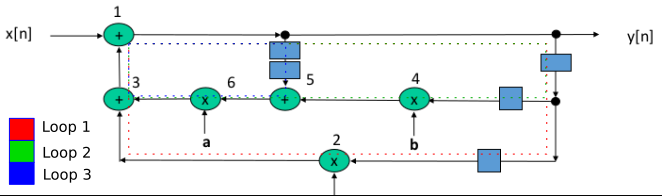
\includegraphics[width=0.8\textwidth]{images/DFGLoop}
	\caption{DFG with Loops labelled}
	\label{fig:images-DFGLoop}
\end{figure}

Each of these loops can be seen to begin and end at the addition node after
the input $x[n]$.

\subsection{Part b}

The stem plot in \ref{fig:Q1Img} shows the stem plot containing both $y[n]$ and
$x[n]$. The values of $x[n]$ are shown to be $\{1,2,3,2,1,1,1,1,1,1,1\}$.

\subsection{Part c}

The computation times for each path, with no delay, are as follows:

\begin{itemize}
	\item Loop 1: 1 Multiplication, 2 Additions
	\begin{itemize}
		\item $2+(2*1)=4$
	\end{itemize}
	\item Loop 2: 2 Multiplications, 3 Additions
	\begin{itemize}
		\item $(2*2)+(3*1)=7$
	\end{itemize}
	\item Loop 3: 1 Multiplication, 3 Additions
	\begin{itemize}
		\item $2+(3*1)=5$
	\end{itemize}
\end{itemize}
Therefore, the critical path is found in the path labelled ``Path 2'' in
Figure \ref{fig:images-DFGLoop}. This path has a length of 7 time units.

\section{Question 2}
\subsection{Part a}

There are 3 loops within this DFG. These loops are indicated below:

\begin{figure}[H]
	\centering
	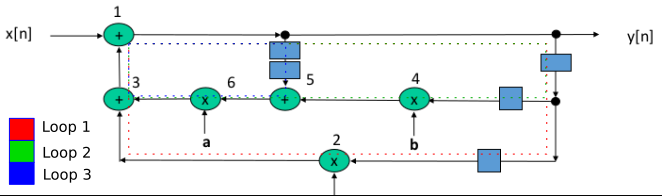
\includegraphics[width=0.8\textwidth]{images/DFGLoop}
	\caption{DFG with Loops labelled}
	\label{fig:images-DFGLoop}
\end{figure}

Each of these loops can be seen to begin and end at the addition node after
the input $x[n]$.

\subsection{Part b}

The stem plot in \ref{fig:Q1Img} shows the stem plot containing both $y[n]$ and
$x[n]$. The values of $x[n]$ are shown to be $\{1,2,3,2,1,1,1,1,1,1,1\}$.

\subsection{Part c}

The computation times for each path, with no delay, are as follows:

\begin{itemize}
	\item Loop 1: 1 Multiplication, 2 Additions
	\begin{itemize}
		\item $2+(2*1)=4$
	\end{itemize}
	\item Loop 2: 2 Multiplications, 3 Additions
	\begin{itemize}
		\item $(2*2)+(3*1)=7$
	\end{itemize}
	\item Loop 3: 1 Multiplication, 3 Additions
	\begin{itemize}
		\item $2+(3*1)=5$
	\end{itemize}
\end{itemize}
Therefore, the critical path is found in the path labelled ``Path 2'' in
Figure \ref{fig:images-DFGLoop}. This path has a length of 7 time units.

\subsection{Part d}

By shifting the register before the addition node ``5'' to between addition node
``5'' and multiplication node ``6'', the following iteration periods are
achieved:

\begin{itemize}
	\item Loop 1:
	\begin{itemize}
		\item 4/2
	\end{itemize}
	\item Loop 2:
	\begin{itemize}
		\item 7/3
	\end{itemize}
	\item Loop 3:
	\begin{itemize}
		\item 5/2
	\end{itemize}
\end{itemize}

Therefore, the iteration period bound has been reduced.
The changes to be made can be seen in Figure \ref{fig:Q3dImg}, found below.

\begin{figure}[H]
	\centering
	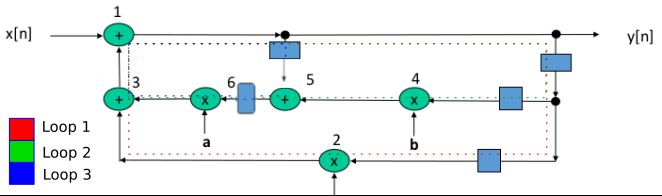
\includegraphics[width=0.8\textwidth]{images/DFGTimedLoop}
	\caption{Retimed DFG}
	\label{fig:Q3dImg}
\end{figure}

\section{Question 3}
\subsection{Part a}

There are 3 loops within this DFG. These loops are indicated below:

\begin{figure}[H]
	\centering
	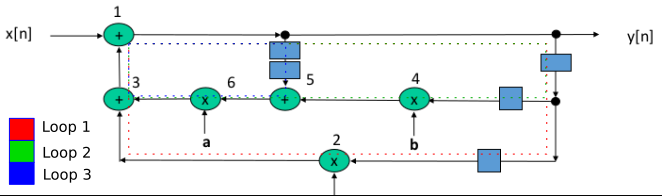
\includegraphics[width=0.8\textwidth]{images/DFGLoop}
	\caption{DFG with Loops labelled}
	\label{fig:images-DFGLoop}
\end{figure}

Each of these loops can be seen to begin and end at the addition node after
the input $x[n]$.

\subsection{Part b}

The stem plot in \ref{fig:Q1Img} shows the stem plot containing both $y[n]$ and
$x[n]$. The values of $x[n]$ are shown to be $\{1,2,3,2,1,1,1,1,1,1,1\}$.

\subsection{Part c}

The computation times for each path, with no delay, are as follows:

\begin{itemize}
	\item Loop 1: 1 Multiplication, 2 Additions
	\begin{itemize}
		\item $2+(2*1)=4$
	\end{itemize}
	\item Loop 2: 2 Multiplications, 3 Additions
	\begin{itemize}
		\item $(2*2)+(3*1)=7$
	\end{itemize}
	\item Loop 3: 1 Multiplication, 3 Additions
	\begin{itemize}
		\item $2+(3*1)=5$
	\end{itemize}
\end{itemize}
Therefore, the critical path is found in the path labelled ``Path 2'' in
Figure \ref{fig:images-DFGLoop}. This path has a length of 7 time units.

\subsection{Part d}

By shifting the register before the addition node ``5'' to between addition node
``5'' and multiplication node ``6'', the following iteration periods are
achieved:

\begin{itemize}
	\item Loop 1:
	\begin{itemize}
		\item 4/2
	\end{itemize}
	\item Loop 2:
	\begin{itemize}
		\item 7/3
	\end{itemize}
	\item Loop 3:
	\begin{itemize}
		\item 5/2
	\end{itemize}
\end{itemize}

Therefore, the iteration period bound has been reduced.
The changes to be made can be seen in Figure \ref{fig:Q3dImg}, found below.

\begin{figure}[H]
	\centering
	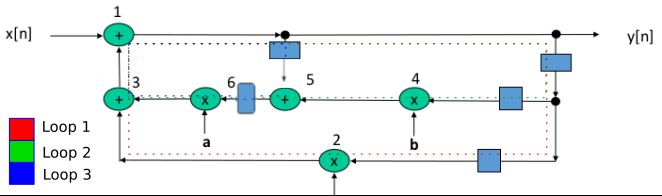
\includegraphics[width=0.8\textwidth]{images/DFGTimedLoop}
	\caption{Retimed DFG}
	\label{fig:Q3dImg}
\end{figure}

\section{Appendix}
\subsection{Question 1}

\lstinputlisting[language=Matlab]{Code/Assignment2/Q1.m}

\subsection{Question 2}

\lstinputlisting[language=Matlab]{Code/Assignment2/Q2.m}

\clearpage
\printbibliography
\end{document}
